\chapter{Les espaces $L^p$}
\section{Définitions}
Dans ce chapitre, on supposera donné un espace mesuré $(E, \mathcal{T}, \mu)$. 
\begin{defn}
Pour $p \geq 1$ réel, l'ensemble $\mathcal{L}^p_{\mathbb{R}}$ (resp.
$\mathcal{L}^p_{\mathbb{C}}$) est l'ensemble des applications $f: E
\to \mathbb{R}$ (resp.  $f: E \to \mathbb{C}$) telles que~:
\[
\int_E |f|^p d \mu < + \infty
\]
L'ensemble  $\mathcal{L}^\infty_{\mathbb{R}}$ (resp.
$\mathcal{L}^\infty_{\mathbb{C}}$) est l'ensemble des applications $f: E
\to \mathbb{R}$ (resp.  $f: E \to \mathbb{C}$) telles que~:
\[
\exists C > 0 \text{ tel que } |f| \leq C \quad \mu\text{-pp}
\]
\end{defn}
Ces ensembles sont des espaces vectoriels sur $\mathbb{R}$ ou
$\mathbb{C}$, mais ne sont pas d'une grande utilité, deux applications
ne différant que sur un ensemble de $\mu$-mesure nulle ayant les mêmes
propriétés vis à vis de l'intégrale. 
Dans la suite, la notation  $\mathcal{L}^p$ désignera selon le
contexte, et si cela ne pose aucune difficulté, aussi bien
$\mathcal{L}^p_{\mathbb{R}}$ que $\mathcal{L}^p_{\mathbb{C}}$.
\begin{prop}
Soit $1 \leq p \leq +\infty$. Dans l'ensemble $\mathcal{L}^p$ la
relation~:
\[
(f \mathcal{R} g) \Leftrightarrow (f = g \quad \mu\text{-pp})
\]
est une relation d'équivalence. La classe d'équivalence de $f$ sera
notée $[f]$.
\end{prop}
\begin{mandatory}
\begin{defn}
Pour $+\infty \geq p \geq 1$, on pose~:
\[
L^p = \mathcal{L}^p / \mathcal{R}
\]
\end{defn}
\end{mandatory}
En vertu de la proposition \ref{ch2:upp}, toutes les applications d'une même
classe d'équivalence ont même intégrale de Lebesgue: on pourra ainsi parler de
l'intégrale d'une classe d'équivalence ou par abus de language de l'intégrale
d'une fonction de $L^p$.

Les ensembles $L^p$ peuvent être munis d'une structure d'espace vectoriel en posant, pour $\mathbb{K} =
\mathbb{R}$ ou $\mathbb{K} = \mathbb{C}$~:
\begin{align*}
& \forall f \in L^p , \, \forall \lambda \in \mathbb{K}, \, \lambda [f] =
  [\lambda f] \\
& \forall f \in L^p, \forall g \in L^p, \, [f] + [g] = [f+g]
\end{align*}


On vérifie également simplement que l'on peut poser, pour toute
application $f \in \mathcal{L}^p$~: $|[f]| = [|f|]$.

Dans la suite, on confondra le plus souvent une classe d'équivalence
avec un représentant, et on parlera de fonction de $L^p$, étant entendu que l'on
travaille en fait sur la classe contenant la fonction.

L'intérêt majeur des espaces $L^p$ est qu'ils peuvent être munis d'une norme.
Pour $f \in L^p, p < +\infty$ (on confond ici comme annoncé représentant avec classes d'équivalence), on posera~:
\[
\| f\|_p = \left ( \int_E |f|^p d \mu \right )^{1/p}
\]
et pour $f\in L^\infty$~:
\[
\|f\|_\infty = \inf \{ C > 0 \text{ tel que } |f(x)| \leq C \mbox{ pour } \mu
\mbox{-presque tout } x \}
\]
On a de façon évidente~:
\begin{itemize}
\item $\|f\|_p = 0 \Leftrightarrow f = 0$. Cette égalité n'est vraie que dans $L^p$ et non dans $\mathcal{L}^p$.
\item $\| \lambda f \|_p = |\lambda| \| f \|$ pour tout $\lambda \in \mathbb{R}$ (resp. $\lambda \in \mathbb{C}$).
\end{itemize}
L'inégalité triangulaire est encore à vérifier, ce qui va être l'objet des développements suivants.
\begin{mandatory}
\begin{theorem}{(Inégalité de Hölder)}
Soit $p \in[1, +\infty]$. Soit $f \in L^p, g\in L^q$ avec $p^{-1}+q^{-1} = 1$ (on dit que $p$ et $q$ sont conjugués). On a~:
\begin{itemize}
\item $fg \in L_1$.
\item $\|fg\|_1 \leq \|f\|_p \|g\|_q$.
\end{itemize}
\end{theorem}
\end{mandatory}
\begin{proof}
Si $p=1, q=\infty$, on écrit simplement~:
\[
\int_E |fg|d \mu \leq \int_E \|g\|_\infty |f| d \mu = \|g\|_\infty \|f\|_1
\]
Supposons donc que $+\infty > p > 1$.
Soit, pour $\alpha \in ]0,1[$, l'application $x>0 \to x^\alpha -
    \alpha x$. Elle est maximale pour $x=1$ d'où~: $\forall x > 0 ,
    x^\alpha - \alpha x \leq 1 - \alpha$.  En considérant un $x$ de la
    forme $\frac{u}{v}$, il vient~:
\[
u^\alpha v^{1-\alpha} \leq \alpha u +(1-\alpha)v
\]
On peut supposer $\|f\|_p>0, \|g\|_q> 0$ car sinon la proposition est évidente.
En prenant $\alpha = p^{-1}$ et~:
\[
\begin{array}{cc}
u = \frac{|f|^p}{\|f\|_p^p} & v = \frac{|g|^q}{\|g\|_q^q}
\end{array}
\]
on a~:
\[
\frac{|fg|}{\|f\|_p\|g\|_q} \leq \frac{|f|^p}{p \|f\|_p^p} +
\frac{|g|^q}{q \|g\|_q^q}
\]
qui conduit par intégration des deux membres de l'inégalité au
résultat recherché.
\end{proof}
L'intérêt de l'inégalité de Hölder va bien au delà de la preuve de l'inégalité
de Minkowsky qui sera vue ci-dessous. Si $p,q$ sont des exposants conjugués,
elle montre que l'intégrale définit sur $L^p \times L^q$ une forme bilinéaire
continue (ou sesquilinéaire continue en complexe).

\begin{mandatory}
 \begin{theorem}{(Inégalité de Minkowsky)}
Soit $p\in [1,+\infty]$ et $f,g \in L^p$. Alors $f+g \in L_p$ et
$\|f+g\|_p \leq \|f\|_p + \|g\|_p$.
\end{theorem}
\end{mandatory}
\begin{proof}
Comme précedemment, les cas $p=1$ et $p=\infty$ sont immédiats. On
supposera donc $+\infty > p > 1$. L'application $x>0 \to x^p$ est
convexe, donc~:
\[
\frac{|f+g|^p}{2^p} \leq \frac{|f|^p + |g|^p}{2}
\]
ce qui prouve que $f+g \in L^p$. En écrivant~:
\[
|f+g|^p =
|f+g||f+g|^{p-1} \leq |f| |f+g|^{p-1} + |g||f+g|^{p-1}
\]
et en intégrant cette inégalité, on obtient~:
\[
\int_E |f+g|^p d \mu \leq \int_E |f||f+g|^{p-1} d \mu + \int_E
|g||f+g|^{p-1} d \mu
\]
L'inégalité de Hölder s'applique aux deux termes du membre de droite avec les
exposants $p,q=p/(p-1)$~:
\[
\int_E |f+g|^p d \mu \leq \|f\|_p \left (\int_E |f+g|^p d \mu \right)
^{\frac{p-1}{p}}
+ \|g\|_p \left (\int_E |f+g|^p d \mu \right )^{\frac{p-1}{p}}
\]
Si $\int_E |f+g|^p d \mu =0$, la proposition est immédiate. Sinon, le
résulat est obtenu en divisant l'inégalité par $ \left (\int_E |f+g|^p d \mu \right )^{\frac{p-1}{p}}$.
\end{proof}
Ce dernier théorème montre que $\|\|_p$ est une norme.
\section{Propriété des espaces $L^p$}
\begin{mandatory}
\begin{theorem}
Munis de la norme $\|\|_p$, les espaces $L^p, p\in [1,+\infty]$ sont complets.
\end{theorem}
\end{mandatory}
\begin{proof}
Le cas $p=\infty$ est simple. Supposons $p < +\infty$. Soit $(f_n)$
une suite de Cauchy dans $L^p$. On peut en extraire une sous-suite
$(g_k)$ telle que $\forall k \in \mathbb{N}, \|g_{k+1}-g_k\|_p \leq
2^{-k}$.
Le théorème de convergence monotone montre immédiatement que~:
\[
\int_E \left ( \sum_{n \geq 1} | g_{n+1} - g_n | \right )^p d
\mu = \lim_{k \to +\infty}  \int_E \left ( \sum_{n=1}^k | g_{n+1} - g_n
| \right )^p d \mu
\]
En appliquant l'inégalité de Minkowsky, le second membre de l'égalité
se majore par~:
\[
\lim_{k \to +\infty}  \left ( \sum_{n=1}^k \| g_{n+1} - g_n \|_p
\right )^p = \left ( \sum_{n \geq 1} \| g_{n+1} - g_n \|_p
\right )^p
\]
qui est une quantité finie.
L'application~:
\[
h = g_1 + \sum_{k\geq 1} (g_{k+1} - g_k)
\]
est donc définie $\mu$-presque partout. Comme $(g_n)$ converge
$\mu$-presque partout vers $h$, le lemme de Fatou donne~:
\[
\int_E |h|^p d \mu \leq \liminf_n \int_E |g_n|^p d \mu 
\]
Le membre de droite est fini car la suite $(g_n)$ est une sous-suite
de la suite $(f_n)$ qui, étant de Cauchy, est bornée.
Ceci prouve que $h \in L^p$. Enfin, pour tout entier $n$~:
\begin{align*}
\int_E | h - g_n|^p d \mu & \leq \liminf_k \int_E |g_k -g_n|^p d \mu
\\
& \leq \left ( \sum_{i=n}^{k-1} \| g_{i+1} - g_i \|_p \right )^p \\
& \leq
\left (2^{-n+1} \right)^p
\end{align*}
qui tend vers 0 pour $n \to +\infty$. On en déduit $g_n \to h$ dans
$L^p$, donc $f_n \to h$ dans $L^p$ et la proposition est prouvée.
\end{proof}
Ce théorème est extrêmement important en pratique et n'a pas
d'équivalent en intégration de Riemann. 
\begin{prop}\label{ch3:p1}
Dans un espace mesuré $(E, \mathcal{T}, \mu)$ avec $\mu(E) < +\infty$,
on a $L^q \subset L^p$ si $1 \leq p \leq q \leq +\infty$.
\end{prop}
\begin{proof}
$\mu$ étant une mesure finie, l'application constante $1$ est sommable
(elle appartient de fait à tous les espaces $L^p$). Soit $f \in
L^p$. L'inégalité de Hölder appliquée au produit $|f|^{p} 1$ donne~:
\begin{align*}
\int_E |f|^p d \mu & \leq \left ( \int_E 1 d \mu \right ) ^{\frac{q}{q-p}}
\|f\|_q \\ & \leq \mu(E)^{\frac{q}{q-p}} \|f\|_q < +\infty
\end{align*}
\end{proof}
\begin{rem}
Rien ne subsiste si $\mu$ n'est pas finie, il faut donc prendre garde à ce que
l'on écrit, comme le montre l'exercice suivant.
\end{rem}
\begin{exercice}
Soit l'application $f : \mathbb{R} \to \mathbb{R}$ définie par~:
\[
\forall x \in \mathbb{R}, \, f(x) = \left \{
\begin{array}{cc}
0 & \mbox { si } < \leq 0 \\
\frac{1}{x(1+ln^2(x))} & \mbox{ sinon }
\end{array}
\right .
\]
\begin{itemize}
\item Montrer que $f$ est sommable.
\item Montrer que $ \forall p > 1, \, f \notin L^p$.
\item En déduire qu'il existe pour tout $p \in [1, +\infty[$ une application $f$ telle que 
$f\in L^p, \, f \notin  L^q, \, q \in  [1, +\infty[, \, q \neq p$.
\end{itemize}
\end{exercice}
Toujours dans le cas des mesures finies, il existe une interprétation de la
notation un peu surprenante $L^\infty$. 
\begin{exercice}
Soit $(E,\mathcal{T},\mu)$ un espace mesuré avec $\mu(E) < +\infty$.
\begin{itemize}
\item Montrer que~:
\[
(f \in L^\infty) \Leftrightarrow \left(\forall p \in [1, +\infty[, \, 
f \in L^p \mbox { et } \sup_p \| f\|_p < +\infty\right)
\]
\item Si ces conditions sont vérifiées, montrer que $\lim_{p \to +\infty}
\|f\|_p = \|f\|_\infty$.
\end{itemize}
\end{exercice}
\begin{theorem}
Pour $p \in [1,+\infty[$, Les applications étagées sont denses dans $L^p$.
\end{theorem}
\begin{proof}
Il suffit de montrer la proposition pour une application $f \in L^p$ réelle positive, le cas
général en decoulant en décomposant une application de $L^p$
quelconque en partie positive et négative (et partie rélle et
imaginaire si $f$ est à valeurs complexes). 
$f$ est limite simple d'une suite croissante $(g_n)$ d'applications étagées
(voir proposition\ref{ch2:1}). Comme pour tout $n$, $g_n \leq f$, on a
également~:
\[
\int_E |g_n|^p d \mu \leq \int_E |f|^p d \mu < +\infty
\]
d'où $\forall n, g_n \in L^p$. Par ailleurs, $\forall n, |f- g_n|^p
\leq 2^p f^p$, donc le théorème de convergence dominée s'applique et l'on
a~:
\[
\lim_n \|f-g_n\|^p = \lim_n \int_E |f - g_n|^p d \mu = 0
\]
\end{proof}
Dans le cas où la mesure $\mu$ vérifie des conditions supplémentaires,
il est possible d'obtenir un résultat de densité pour des applications
plus régulières que les applications étagées.  
\begin{prop}
Soit $E$ un espace métrique muni de sa tribu des Boréliens et
  soit $\mu$ une mesure vérifiant la propriété~:
\[
\forall A \in \mathcal{B}(E), \, \mu(A) = \inf \{ \mu(O), O \mbox{
  ouvert }, \, O \supset A \}
\]
alors l'ensemble des applications lipschitziennes bornées est dense dans
$L^p(E, \mathcal{B}(E), \mu)$.
\end{prop}
\begin{proof}
On peut se limiter à prouver que toute indicatrice $1_A$ avec $A \in
\mathcal{B}(E)$  est limite dans $L^p$ d'une suite
d'applications lipschitiziennes bornées. 
Soit $\epsilon > 0$. Il existe par hypothèse un ouvert $O$ tel que $O
\supset a$ et $\mu(O-A) < \epsilon$. On en déduit~:
\[
\| 1_O - 1_A \|_p^p < \epsilon
\]
Soit pour tout entier $k$ l'application lipschitzienne ~: 
\[
g_k(x) = \min(k d(x, O^c), 1) 
\]
On a $\lim g_k \to 1_O$ et, par le théorème de convergence dominée~:
\[
\lim_k \int_E |1_O -g_k|^p d \mu \to 0
\]
donc il existe $k_0$ tel que~:
\[
\forall k \geq k_0 \, , \, \| 1_0 - g_k \|_p^p < \epsilon
\]
La suite $(g_k)$ converge ainsi dans $L^p$ vers $1_A$ et la proposition est prouvée.
\end{proof}
\section{L'espace $L^2$}
L'exposant $2$ est conjugué à lui-même. La forme bilinéaire (resp.
sesquilinéaire) donnée par l'inégalité de Hölder va induire un produit scalaire
sur cet espace. Associé à la complétude, le caractère Hilbert de $L^2$
s'ensuivra.
\begin{mandatory}
\begin{prop}
L'espace $L^2$ muni du produit scalaire~:
\[
\langle f, g \rangle = \int_E f \overline{g} d \mu
\]
est un espace de Hilbert.
\end{prop}
\end{mandatory}
Le caractère Hilbert de $L^2$ permet d'utiliser quelques théorèmes très
puissants comme l'existence d'une projection orthogonale ou le théorème de
représentation de Riesz. Ces deux résultats sont rappelés ci-dessous:
\begin{mandatory}
\begin{theorem}
Soit $H$ un espace de Hilbert et soit $C \subset H$ une partie convexe fermée
non vide de $H$. Pour tout $x \in H$, il existe un unique point $\tilde{x} \in
C$ tel que $\forall y \in C, \, \|x-\tilde{x}\| \leq \|x-y\|$. 
Dans le cas où $C$ est un sous-espace vectoriel fermé de $H$, ce point est
caractérisé par la propriété suivante:
\[
\forall y \in C, \, \langle x - \tilde{x}, y - \tilde{x}\rangle=0
\]
\end{theorem}
\end{mandatory}
La démonstration n'est pas rappelée ici, mais utilise une suite de Cauchy
de points de $C$ convergeant vers $\tilde{x}$: le caractère fermé et complet de
$C$ est absolument nécessaire. Le point $\tilde{x}$ est appelé projection
orthogonale de $x$ sur $C$.
\begin{mandatory}
\begin{theorem}(Théorème de représentation de Riesz)
Soit $H$ un espace de Hilbert et soit $\phi \colon H \to \mathbb{R}$ (resp.
$\phi \colon H \to \mathbb{C}$) une forme linéaire \textbf{continue} sur $H$. Il
existe un unique vecteur $v \in H$ tel que:
\[
\forall x \in H, \, \phi(x) = \langle x, v \rangle
\]
\end{theorem}
\end{mandatory}
\begin{proof}
La forme $\phi$ étant continue, son noyau $\ker \phi = \phi^{-1}(0)$ est un
sous-espace vectoriel fermé de $H$. Pour tout $x\in H$, on note $p(x)$ sa
projection orthogonale sur $\ker \phi$ (elle existe en vertu du théorème
précédent). L'écriture $x = (x-p(x)) + p(x)$ montre que $\ker \phi$ possède un
supplémentaire orthogonal $H_1$ dans $H$. $H_1$ est de dimension $1$
($\phi|_{H_1}$ est inversible), donc est engendré par un vecteur non nul $e$
tel que $\phi(e) \neq 0$. Pour tout $x \in H$, peut ainsi écrire $x = \lambda e
+ y$, $y \in \ker \phi$ et $\lambda$ un scalaire. On note que $\phi(x) =
\lambda \phi(e)$ et que $\langle x, e,\rangle  = \lambda \langle e, e \rangle$.
Le vecteur $v$ de la proposition est donc:
\[
v = e \frac{\phi(e)}{\langle e, e \rangle}
\]
\end{proof}
Le théorème de représentation de Riesz, appliqué à $L^2$, permet de prouver de
façon élégante un résultat d'une grande importance en théorie des probabilités.
\begin{defn}
Soit $(E, \mathcal{T})$ un espace mesurable et soient $\mu, \nu$ deux
mesures sur $E$. On dira que $\nu$ est absolument continue par rapport
à $\mu$ (noté $\nu \ll \mu$) si pour toute partie $A \in \mathcal{T}$,
$\mu(A) = 0 \Rightarrow \nu(A) = 0$. De même, on dira que $\nu$ est
étrangère à $\mu$ (noté $\nu \perp \mu$) si il existe $A \in
\mathcal{T}$ avec $\mu(A) = 0$ et $\nu(A^c) = 0$.
\end{defn}
Une forme très importante de mesure absolument continue est donnée par la proposition ci-dessous.
\begin{mandatory}
\begin{prop}
Soit $(E, \mathcal{T}, \mu)$ un espace mesurable
et soit  $f$ une application positive sommable définie sur $E$. On pose pour
tout $A$ mesurable:
\[
\mu_f(A) = \int_{A} f(x) d \mu(x)
\]
Alors $\mu_f$ est une mesure absolument continue par rapport à $\mu$.
\end{prop}
\end{mandatory}
\begin{proof}
$\mu_f(\emptyset)=0$ de façon évidente et si $(A_n)_{n \in \mathbb{N}}$ est une
famille disjointe de parties $\mu$-mesurables, alors:
\[
\mu_f\left(\bigcup_{n \in \mathbb{N}} A_n \right) = \int_{\mathbb{R}} \sum_{n
\in \mathbb{N}} 1_{A_n} f(x) d \mu(x)
\]
Par le théorème de convergence dominée, il vient:
\[
 \int_{\mathbb{R}} \sum_{n
\in \mathbb{N}} 1_{A_n} f(x) d \mu(x) = \lim_{k \to +\infty}
\int_{\mathbb{R}} \sum_{n=0}^k 1_{A_n} f(x) d \mu(x)
\]
Soit avec la relation de Chasles:
\[
\int_{\mathbb{R}} \sum_{n
\in \mathbb{N}} 1_{A_n} f(x) d \mu(x) = \lim_{k \to +\infty}
\sum_{n=0}^k \int_{A_n} f(x) d \mu(x) = \lim_{k \to +\infty}
\sum_{n=0}^k \mu_f(A_n)
\]
qui prouve l'additivité dénombrable.
Soit $\epsilon > 0$. Le théorème de convergence monotone donne:
\[
\lim_{n \to +\infty} \int_{\mathbb{R}} f\wedge n(x) d \mu(x) = 
\int_{\mathbb{R}} f(x) d \mu(x)
\] 
Il existe donc $n_\epsilon$ tel que pour tout $n \geq n_{\epsilon}$:
\[
\int_{\mathbb{R}} f(x) d \mu(x) - int_{\mathbb{R}} f\wedge n(x) d \mu(x)
< \frac{\epsilon}{2}
\]
Soit $A$ une partie $\mu$-mesurable telle que:
$$\mu(A) < \frac{\epsilon}{2n_\epsilon}$$
On a, pour tout $n \geq n_{\epsilon}$:
\[
\int_{A} f(x)d \mu(x) < \int_{A} f \wedge n(x) d \mu(x) +
\frac{\epsilon}{2} < n \mu(A) + \frac{\epsilon}{2}  < \epsilon
\]
\end{proof}
Le théorème de Radon-Nikodym énoncé ci-dessous va établir une forme de
réciproque.
\begin{mandatory}
\begin{theorem}{(Radon-Nikodym)}
Soit $\mu, \nu$ deux mesures $\sigma$-finies sur un espace mesurable $(E,
\mathcal{T})$. Il existe un unique couple $(\nu_a, \nu_s)$ de mesures
finies sur $(E, \mathcal{T})$ tel que~:
\begin{itemize}
\item $\nu = \nu_a + \nu_s$;
\item $\nu_a \ll \mu, \, \nu_s \perp \mu$;
\item $\nu_a = f \mu$, $f$ application sommable sur
$E$.
\end{itemize}
\end{theorem}
\end{mandatory}
\begin{proof}
On suppose dans un premier temps que les mesures sont finies et que
pour toute application positive sommable $f$~: 
\[
\int_E f d \nu \leq \int_E f d \mu
\]
Pour $f \in L^2(\mu)$, on pose~:
\[
P(f) = \int_E f d \nu
\]
Cette quantité est bien définie car $\nu$ finie implique $L^2(\nu) \subset
L^1(\nu)$ en vertu de la proposition \ref{ch3:p1} et par hypothèse~:
$\|f\|_{L^2(\nu)} \leq \|f\|_{L^2(\mu)}$. Par ailleurs,
l'inégalité de Hölder donne~:
\[
|P(f)| \leq \sqrt{\nu(E)} \|f\|_{L^2(\mu)}
\]
$P$ est donc une forme linéaire continue sur $L^2(\mu)$, espace de
Hibert. Le théorème de représentation de Riesz montre qu'il existe une
application $g \in L^2(\mu)$ telle que ~:
\[
\forall f \in L^2(\mu), \, P(f) = \int_E f g  d \mu
\]
et l'on a, pour toute partie mesurable $A$~:
\[
\nu(A) = \int_E 1_A g d \mu
\]
L'application $g$ peut être choisie de telle sorte qu'elle prenne ses
valeurs dans $[0,1]$. En effet, pour tout $\epsilon > 0$~:
\begin{align*}
&\nu(\{x | g(x) < - \epsilon \})
\leq -\epsilon \mu(\{x| g(x) < - \epsilon \}) \\
&\mu(\{x | g(x) > 1 + \epsilon \}) \geq \nu(\{x | g(x) > 1 + \epsilon
\}) \geq \\
& (1+\epsilon) \mu(\{x | g(x) > 1 + \epsilon \})
\end{align*}
d'où~:
\[
\mu(\{x | g(x) < - \epsilon \}) = \mu(\{x | g(x) > 1 + \epsilon \}) = 0
\]
En revenant au problème initial et toujours dans l'hypothèse de
mesures finies, on peut appliquer le développement
précédent aux mesures $\nu, \nu+\mu$. Pour toute application mesurable
bornée $f$ il existe une application $g$ avec~:
\[
\int_E f d \nu = \int_E f g d \mu + \int_E f g d \nu
\]
soit~:
\[
\int_E f (1-g) d \nu = \int_E fg d \mu 
\]
résultat s'étendant à toute appplication mesurable positive par le
théorème de convergence monotone. 
L'ensemble $N = \{ x | g(x) = 1 \}$ est de $\mu$-mesure nulle (faire
$f=1_N$ dans l'égalité précédente). On obtient alors les mesures~:
\begin{align*}
& \nu_s = 1_N \nu \\
& \nu_a = 1_{N^c} \nu
\end{align*}
avec, pour tout $A$ mesurable~:
\[
\nu_a(A) = \int_E 1_{A \cap N^c} \frac{g}{1-g} d \mu
\]
L'unicité s'obtient de façon simple. Pour le cas $\sigma$-fini,
appliquer le résultat précédent sur un recouvrement dénombrable de $E$ par des
ensembles de mesure finie.
\end{proof}
Enfin, il faut terminer ce développement en mentionnant la relation existant
entre intégrale et primitive dans le cadre de la théorie de Lebesgue.
\begin{mandatory}
\begin{theorem}\label{thm:derivee_integrale}
Soit $f$ une application sommable. On pose pour tout $x \in \mathbb{R}$:
\[
F(x) = \int_{]-\infty,x]} f(t) d \lambda(t)
\]
alors pour presque tout $x \in \mathbb{R}$, l'application $F$ est dérivable en
$x$ de dérivée est égale à $f(x)$.
\end{theorem}
\end{mandatory}
Cette proposition justifie le calcul d'une intégrale par une primitive, sous
réserve bien sûr qu'elle puisse être exhibée dans ce cadre plus général. La
preuve de cet énoncé simple en apparence est étonnamment difficile. Plusieurs
lemmes intermédiaires sont nécessaires avant de pouvoir conclure. Le premier est
dû à F. Riesz et porte le nom évocateur de lemme du soleil levant.
\begin{lemme}\label{lem:soleil_levant}
Soit $f : \mathbb{R} \to \mathbb{R}$ une application continue telle que
$\lim_{x \to +\infty} f(x) = - \infty$, $\lim_{x \to -\infty} f(x) = +\infty$.
L'ensemble:
\[
\mathcal{A} = \{ x | \exists y > x , f(y) > f(x) \}
\]
est ouvert et s'écrit sous la forme d'une union dénombrable d'intervalles
ouverts bornés:
\[
\mathcal{A} = \cup_{i \in \mathbb{N}} ]a_i,b_i[
\]
avec $f(a_i)=f(b_i)$ pour tout entier $i$.
\end{lemme}
Le nom du lemme provient du fait que l'ensemble $\mathcal{A}$ contient tous les
points du graphe de $f$ qu'un observateur situé en $+\infty$ ne pourrait pas
voir, car masqués par d'autres points ou encore tous les points qui ne seraient
pas éclairés par le soleil levant ! La situation décrite par le lemme est
représentée en figure \ref{fig:rising_sun}

\begin{center}
\begin{figure}[ht]
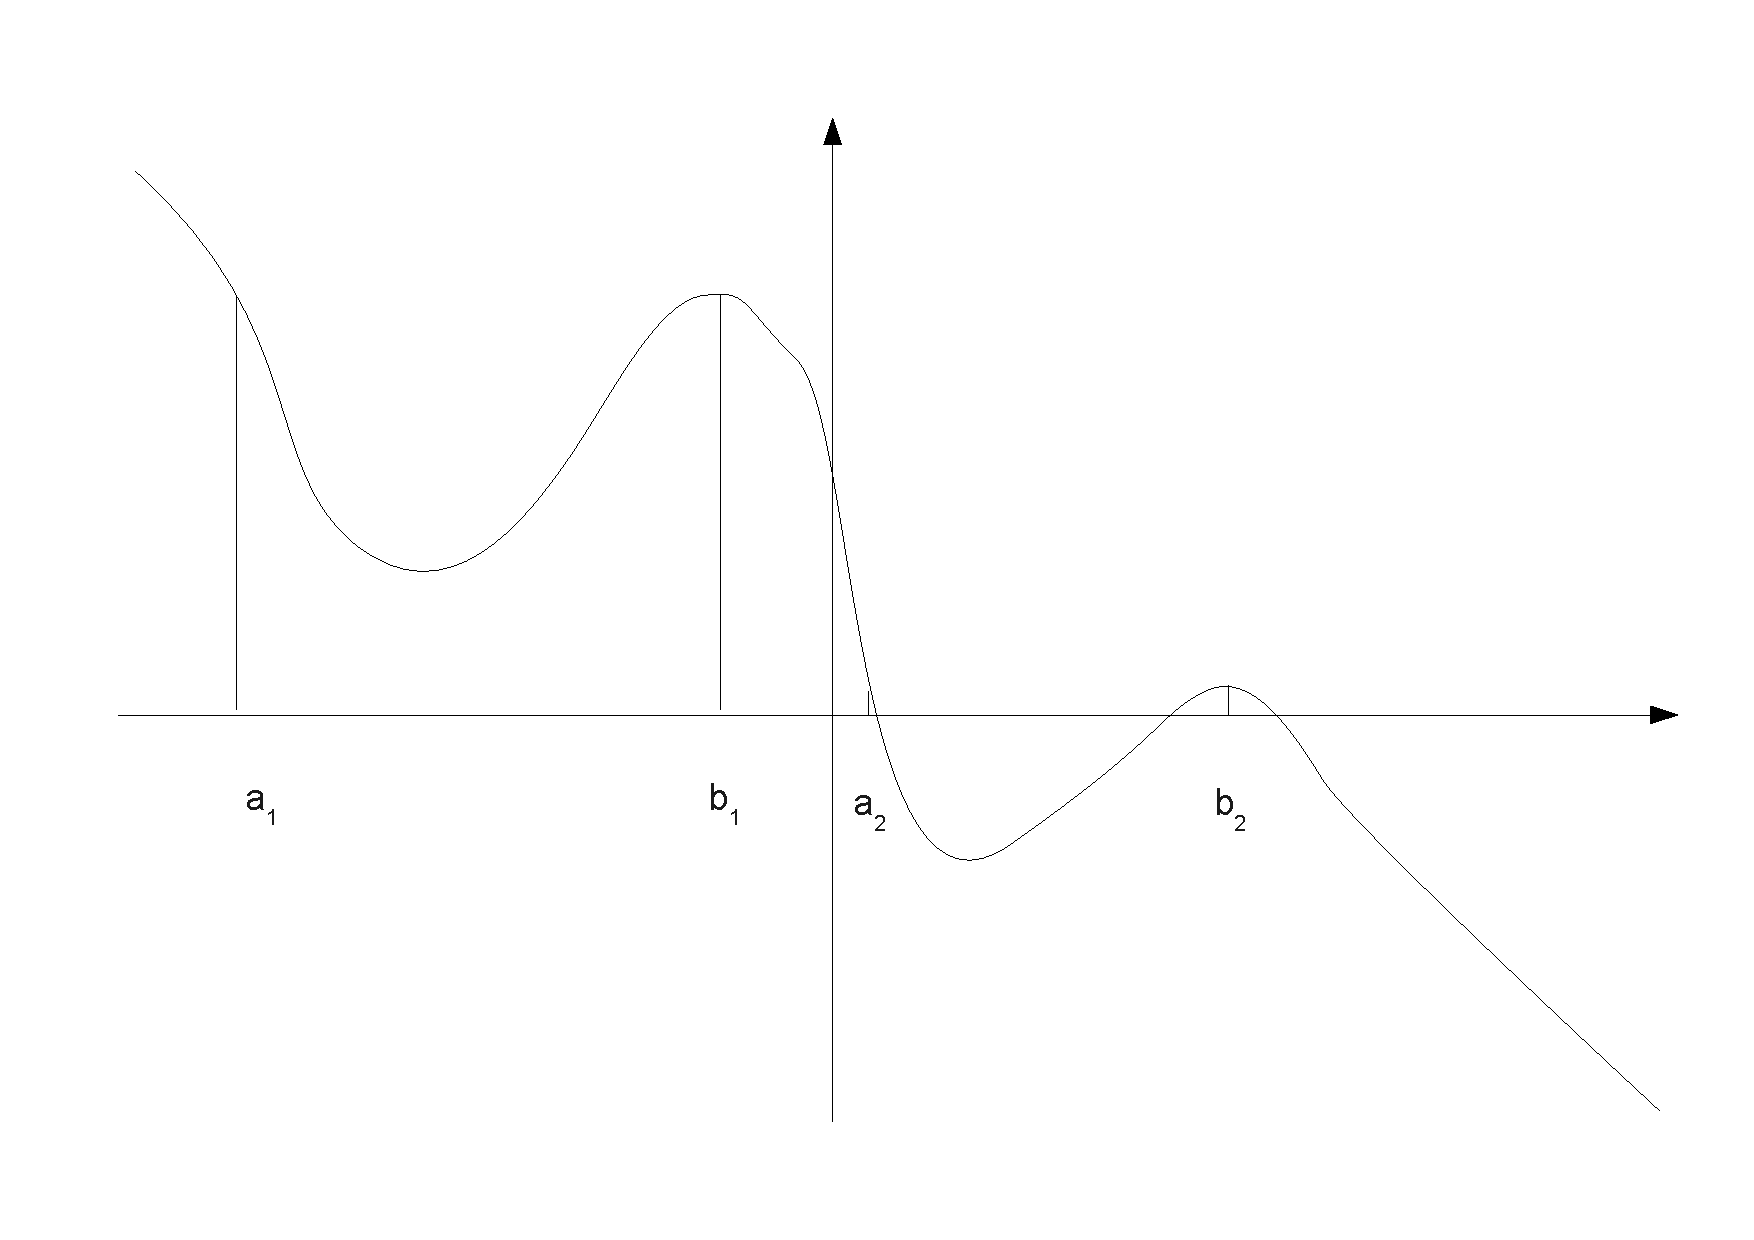
\includegraphics[scale=0.3]{images/rising_sun.pdf}
\caption{Lemme du soleil levant}\label{fig:rising_sun}
\end{figure}
\end{center}

\begin{proof}
Montrons en premier lieu que $\mathcal{A}$ est ouvert. Soit $x \in \mathcal{A}$.
Il existe $y > x$ tel que $f(y) > f(x)$. Soit $\delta = f(y)-f(x)$.
Les points de l'intervalle $I=]f(x)-\delta/2, f(x)+\delta/2[$ sont inférieurs à
$f(y)$. Par continuité de $f$ en $x$, il existe un intervalle ouvert
$J=]x-\epsilon, x+\epsilon[$ tel que $f(J) \subset I$. Quite à réduire
$\epsilon$, on peut supposer que tous les points de $J$ sont inférieurs à $y$ et
on a $J \subset \mathcal{A}$ prouvant que ce dernier ensemble est ouvert. Un
résultat de topologie déjà mentionné montre qu'il s'écrit sous la forme d'une
union dénombrable d'intervalles ouverts, la démonstration du lemme se réduit
alors à pouver qu'ils sont tous bornés. Supposons l'existence d'un intervalle
de la forme $]a,+\infty[ \subset \mathcal{A}$. Soit $K$ un réel. Comme $f$ tend
vers $-\infty$ en $+\infty$, il existe un réel $M>a$ tel que pour tout $x > M$ on ait $f(x) <
f(a)-1$. L'ensemble $\{ u > a, \forall x > u, f(x) < f(a)-1\}$ est non vide (il
contient $M$) et admet une borne inférieure $t$. Pour tout $\epsilon > 0$, on a
$f(t+\epsilon) < f(a) - 1$  et par continuité de $f$, $f(t) \leq f(a)-1$, d'où
$t> a$. Par ailleurs:
\[
\forall x \geq t, f(x) \leq f(a)-1
\] 
et donc $t \notin \mathcal{A}$ ce qui est une
contradiction.
Supposons maintenant qu'un intervalle $]-\infty, a[$ soit inclus dans
$\mathcal{A}$. Comme $f$ est continue et a pour limite $-\infty$ en $+\infty$,
il existe un réel $M$ tel que pour tout $x \geq a$ on ait $f(x) < M$. L'ensemble
des $u$ tels que $f(u) \geq M$ est non vide, contenu dans l'intervalle
$]-\infty, a[$. Soit $t$ sa borne inférieure. Par continuité de $f$, $f(t) = M$
et donc $t < a$. Comme par ailleurs:
\[
\forall x > t, f(x) \leq f(t) 
\]
on aboutit à une contradiction.
Finalement, soit $]a,b[$ un intervalle contenu dans $\mathcal{A}$. Par
définition, $a$ n'appartient pas à $\mathcal{A}$ et on a donc $f(a) \geq f(b)$.
Supposons qu'il existe $t$ dans $]a,b[$ tel que $f(t) > f(b)$. Comme $t$ est
dans $\mathcal{A}$, il existe $y > t$ tel que $f(t) < f(y)$. L'ensemble:
\[
\{ y , y > t, f(t) < f(y) \}
\]
est donc non vide. Il est borné car $f$ tend vers $-\infty$ en $+\infty$ et
admet donc une borne supérieure $g$ finie. Par continuité de $f$, $f(g)=f(t)$ et
pour tout $y > g$, on a $f(y) \leq f(g)$. On en déduit que $g \notin
\mathcal{A}$ et donc que $g > b$. Or $f(g)=f(t)> f(b)$, donc $b \in \mathcal{A}$
ce qui est une contradiction. Ceci montre que pour tout $t \in ]a,b[$, $f(t)
\leq f(b)$ et donc par continuité de $f$, $f(a) \leq f(b)$, soit $f(a)=f(b)$.
 \end{proof}
Le lemme suivant est simple à prouver, mais très utile, spécialement en
probabilités et statistique.
\begin{lemme}{Inégalité de Markov}\label{lem:ineg_markov}
Soit $f$ une fonction de $L^1(\mu)$. Pour tout $\epsilon > 0$, on a:
\[
\mu \left \{ x , |f(x)| > \epsilon 
\right \} \leq \frac{\|f\|_{L^1(\mu)}}{\epsilon}
\] 
\end{lemme}
\begin{proof}
La démonstration est très classique et aisée.
On a:
\begin{align*}
\|f\|_{L^1(\mu)} &= \int_{\mathbb{R}}|f(x)| d\mu(x)  \\
& \geq \int_{\left \{ x , |f(x)| > \epsilon \right \}}|f(x)| d\mu(x) > \epsilon
\mu \left \{ x , |f(x)| > \epsilon \right \}  
\end{align*}
La majoration demandée s'en déduit immédiatement. 
\end{proof}
Le dernier ingrédient est une majoration que l'on appelle inégalité de
Hardy-Littlewood. Elle s'applique à une fonction qui représente une
moyenne sur des intervalles: la fonction maximale de Hardy-Littlewood.
\begin{defn}\label{def:hardy_littlewood}
Soit $f \in L^1$. La fonction maximale de Hardy-Littlewood est définie pour tout
$x$ réel comme:
\[
Mf(x) = \sup_{x \in [a,b]} \frac{1}{b-a} \int_{]a,b[} |f(t)| dt
\]
où la borne supérieure est prise sur tous les intervalles contenant $x$.
\end{defn}
\begin{prop}\label{prop:ineg_hardy_littlewood}
Soit $f \in L^1$. Pour tout $\epsilon > 0$:
\[
\lambda \left(\{ x, Mf(x) \geq \epsilon \}\right) \leq \frac{2}{\epsilon}
\|f\|_{L^1}
\]
\end{prop}
Cette proposition est semblable à l'inégalité de Markov, mais demande un peu
plus de travail pour sa preuve. On utilisera le lemme du soleil levant.
\begin{proof}
On note en premier lieu que le problème se simplifie par l'introduction des
fonctions maximales positives et négatives:
\[
M^+f(x)= \sup_{h > 0} \frac{1}{h} \int_x^{x+h} |f(t)| dt, \, M^-f(x)= \sup_{h >
0} \frac{1}{h} \int_{x-h}^x |f(t)| dt
\]
Il est clair que:
\[
\{x , Mf(x) \geq \epsilon \} = \{x , M^+f(x) \geq \epsilon \}\cup \{x , M^-f(x)
\geq \epsilon \}
\]
On va utiliser $M^+f$, le même raisonnement s'appliquant à $M^-f$. Par
définition, si $M^+f(x) > \epsilon$ alors il existe un $h > 0$ tel que:
\[
\int_x^{x+h} |f(t)| dt > \epsilon h
\]
Soit la fonction:
\[
F_\epsilon \colon u \mapsto \int_{]-\infty,u[} |f(t)|dt - \epsilon u
\]
Elle vérifie les conditions du lemme \ref{lem:soleil_levant} (le vérifier !) et
on a $F_\epsilon(x+h) > F_{\epsilon}(x)$. Soit l'ensemble:
\[
\mathcal{A}_\epsilon = \{ x, \exists y > x, F_\epsilon(y) > F_\epsilon(x) \} 
\]
Par le lemme \ref{lem:soleil_levant}, cet ensemble s'écrit comme réunion
dénombrable disjointe d'intervalles ouverts bornés:
\[
\mathcal{A}_\epsilon = \bigcup_{k \in \mathbb{N}}]a_k,b_k[
\]
avec $F_\epsilon(a_k)=F_\epsilon(b_k)$. Cette dernière égalité implique:
\[
\int_{a_k}^{b_k} |f(t)|dt = \epsilon (b_k - a_k)
\]
Evaluons la mesure de $\mathcal{A}_\epsilon$:
\begin{align*}
\lambda \left (\mathcal{A}_\epsilon \right) & = \sum_{k \in \mathbb{N}} b_k -
a_k
\\
&= \frac{1}{\epsilon} \sum_{k \in \mathbb{N}} \int_{a_k}^{b_k}|f(t)|dt \\
& \leq \frac{1}{\epsilon}\|f\|_{L^1}
\end{align*}
Or:
\[
\{x , M^+f(x) > \epsilon \} \subset  \mathcal{A}_\epsilon
\]
d'où:
\[
\lambda \left( \{x , M^+f(x) > \epsilon \} \right) \leq
\frac{1}{\epsilon}\|f\|_{L^1}
\]
L'expression est continue en $\epsilon$, on peut passer à l'inégalité large:
\[
\lambda \left( \{x , M^+f(x) \geq \epsilon \} \right) \leq
\frac{1}{\epsilon}\|f\|_{L^1}
\]
et le résultat demandé s'en déduit (même calcul pour $M^-f$).
\end{proof}
Il est maintenant possible de prouver le théorème \ref{thm:derivee_integrale}.
\begin{proof}
Soit $\epsilon > 0$ et soit l'ensemble:
\[
G_\epsilon  = \{ x, \limsup_{h \to 0}\frac{1}{h} \int_x^{x+h} | f(t) - f(x) |
dt >
\epsilon
\}
\]
L'ensemble des fonctions continues étant denses dans $L^1$, pour tout $\eta >
0$, il existe $g_\eta$ continue telle que $\|f-g_\eta\|_{L^1} < \eta$. On a:
\begin{align*}
 \limsup_{h \to 0} \int_x^{x+h} | f(t) - f(x) | dt & = \limsup_{h \to 0}
 \frac{1}{h} \int_x^{x+h} | f(t) - g_\eta(t) | dt  \\
 & + \limsup_{h \to 0} \frac{1}{h}
 \int_x^{x+h} | g_\eta(t) - g_\eta(x) | dt \\
 & + \limsup_{h \to 0} \frac{1}{h}
 \int_x^{x+h} | g_\eta(x) - f(x) | dt
\end{align*}
$g_\eta$ étant continue, le second terme du membre de droite est nul. Par
ailleurs, le troisième terme est égal à $| g_\eta(x) - f(x) |$ et le premier est
inférieur ou égal à la fonction maximale de $f-g_\eta$.
On a:
\[
G_\epsilon  \subset \{x , | g_\eta(x) - f(x) | \geq \epsilon / 2 \} \cup \{
M(f-g\eta)(x) \geq \epsilon / 2 \}
\]
La mesure du premier ensemble du membre de droite se majore par l'inégalite
\ref{lem:ineg_markov} et la seconde par Hardy-Littlewood. Au total, il vient:
\[
\lambda \left(G_\epsilon\right) \leq \frac{2\eta}{\epsilon} + \frac{4
\eta}{\epsilon}
\]
Cette quantité tendant vers 0 pour $\eta$ tendant vers 0, on en déduit $\lambda
\left(G_\epsilon\right) = 0$.
En écrivant:
\[
\lambda\left(\bigcup_{k
\in \mathbb{N}} G_{k^{-1}} \right ) = \lim_{k \to +\infty} \lambda\left(
G_{k^{-1}} \right ) = 0
\]
on a finalement:
\[
\lambda \left (
\{ x, \limsup_{h \to 0}\frac{1}{h} \int_x^{x+h} | f(t) - f(x) |
dt > 0
\}
\right ) =0
\]
Ce qui montre que l'on a presque partout:
\begin{align*}
\limsup_{h \to 0} \left | \frac{F(x+h)-F(x)}{h} - f(x) \right | & \leq
\limsup_{h \to 0}\frac{1}{h} \int_x^{x+h} | f(t) - f(x) | dt \\
&  = 0
\end{align*}
qui est bien la conclusion du théorème.
\end{proof}

Le théorème fondamental de l'analyse prouve que l'intégrale d'une dérivée est
bien égale à la fonction de départ à une constante additive. Il est également
délicat à prouver.
De plus, l'exemple de la fonction de Cantor ou "escalier du diable" ci-dessous
montre que des hypothèses supplémentaires sur l'application à intégrer sont
nécessaires. Cette application est construite sur l'intervalle $[0,1]$ comme
limite uniforme d'une suite d'applications $(f_n)_{n \in \mathbb{N}}$:
\begin{itemize}
  \item $f_0 \colon x \mapsto x$.
  \item Par récurrence, $f_{n+1}$ est définie à partir de $f_n$:
  \[
  f_{n+1} \colon x \mapsto \left \{ 
  	\begin{array}{cc}
  		\rule[-0.5em]{0pt}{2em} \frac{1}{2} f_n(3x) & x \in
  		 \left[0, \frac{1}{3}\right[ \\ 
  		 \rule[-0.5em]{0pt}{2em} \frac{1}{2} & x \in \left[\frac{1}{3},
  		\frac{2}{3}\right[ \\ 
  		\rule[-0.5em]{0pt}{2em} \frac{1}{2}f_n(3x-2)+ \frac{1}{2} & x \in
  		\left[\frac{2}{3}, \frac{2}{3}\right]
  	\end{array}
  \right.
  \]
\end{itemize}
La suite $(f_n)_{n \in \mathbb{N}}$ converge uniformément vers une application
continue $f$ que l'on appelle fonction de Cantor (voir figure \ref{ch6:fig1}). 
\begin{figure}[hb]
\begin{center}
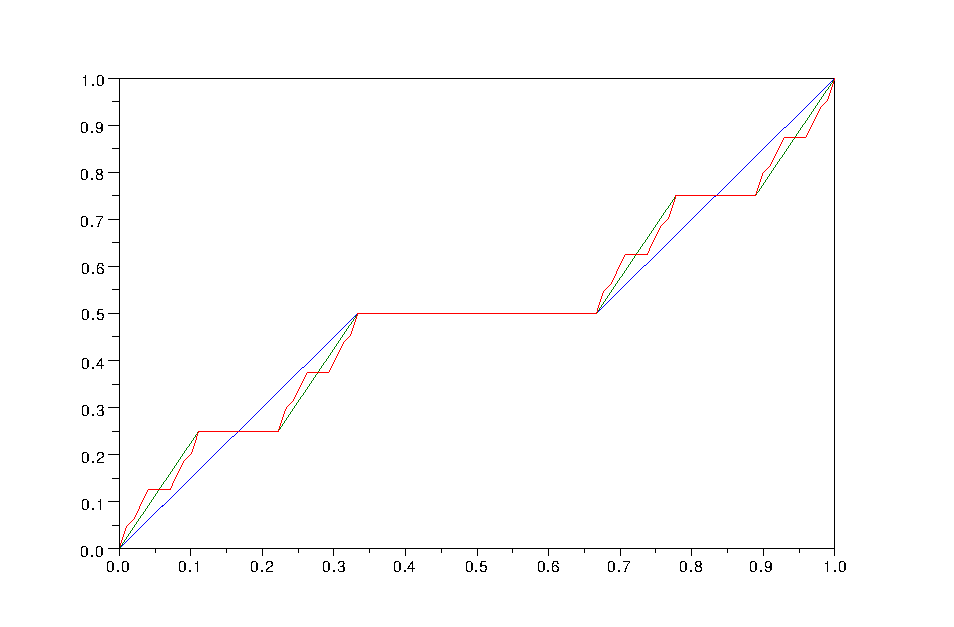
\includegraphics[scale=0.5]{images/cantor.pdf}
\caption{Fonction de Cantor}\label{ch6:fig1}
\end{center}
\end{figure}
$f$ sera
dérivable en tout point $x$ tel que dans son développement en base $3$, $x=\sum_{n \in \mathbb{N}}
a_i 3^{-i}$, il existe un $a_i$ de valeur $1$ et au moins un $a_j, j > i$ non
nul (on vérifiera que cette condition signifie que $x$ appartient à un
intervalle ouvert sur lequel l'une des fonctions $f_n$ est constante). Sur tous
ces points, la dérivée de $f$ est nulle. Le complémentaire de ces points est une
intersection dénombrable d'ensembles fermés (voir figure \ref{ch6:fig2}), donc
mesurable, et un calcul élémentaire de limite montre que sa mesure est nulle (vérifier sur la
figure \ref{ch6:fig2} que la mesure de $F_n$ est $\frac{2^n}{3^n}$). On en déduit que
$f^\prime$ existe pour presque tout $x$, mais aussi que pour tout $x \in [0,1]$:
\[
\int_{[0,x]} f^\prime(t) d \lambda(t) = 0 \neq f(x)
\]
\begin{figure}[hb]
\begin{center}
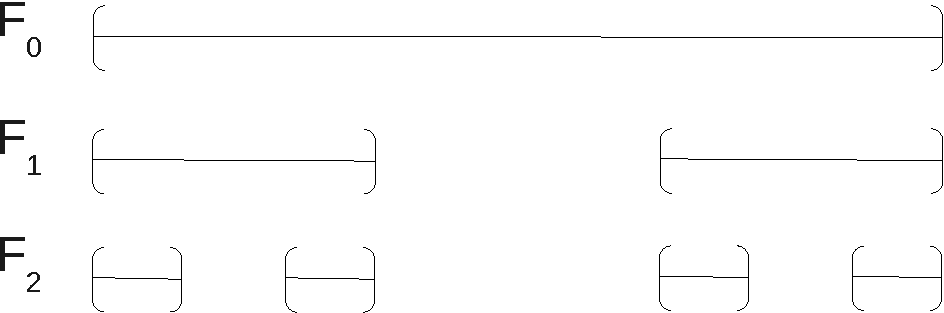
\includegraphics[scale=0.5]{images/ens_cantor.pdf}
\caption{Ensemble de Cantor}\label{ch6:fig2}
\end{center}
\end{figure}
La fonction de Cantor est un cas particulier d'une application singulière:
\begin{defn}
Une application $f$ définie sur $\mathbb{R}$ est dite singulière si elle est
dérivable en presque tout point et de dérivée nulle.
\end{defn}
Une application singulière ne peut pas être égale à l'intégrale de sa
dérivée.
\begin{defn}
Soit $F \colon [a,b] \to \mathbb{R}$. On dira que $F$ est absolument continue
pour tout $\epsilon > 0$ il existe un $\delta > 0$ telle que pour toute famille
finie d'intervalles $]a_i, b_i[, i = 1, \dots, n$:
\[
\sum_{i=1}^n (b_i - a_i) < \delta \Rightarrow \sum_{i=1}^n
\left(F(b_i)-F(a_i)\right) < \epsilon
\]
\end{defn}
\begin{mandatory}
\begin{theorem}{(Théorème fondamental de l'analyse)}
Soit $F$ une application absolument continue sur un intervalle $[a,b]$. Alors
$F$ est dérivable sauf sur un ensemble de mesure de Lebesgue nulle. Si
$f=F^\prime$ $\lambda$-presque partout, alors $f$ est sommable et pour tout $x
\in [a,b]$:
\[
F(x) = F(a) + \int_{[a,x]} f(t) d \lambda(t)
\]
\end{theorem}
\end{mandatory}
Ce théorème  repose sur le lemme de Vitali.
\begin{defn}
Soit $A$ une partie de $\mathbb{R}$. Un recouvrement de Vitali de $A$ est une
famille d'intervalles fermés $([a_i,b_i])_{i \in \mathbb{N}}$ telle que pour
tout $x \in A$ et pour tout $\epsilon > 0$ il existe un intervalle $[a_j,b_j]$
contenant $x$ tel que $b_j-a_j < \epsilon$.
\end{defn}
\begin{lemme}{(Lemme de Vitali)}
Soit $A$ une partie mesurable de $\mathbb{R}$ de mesure de Lebesgue finie. Soit
$\mathcal{V}$ un recouvrement de Vitali de $A$ par des intervalles de longueur
bornée par $M >0$. Pour tout $\epsilon > 0$, il existe une famille disjointe
finie $(I_i)_{i=1, \dots, n}$ d'intervalles de $\mathcal{V}$ telle que:
\[
\sum_{i=1}^n \lambda(I_i) \geq \lambda(A) - \epsilon
\]
\end{lemme}
\begin{proof}
On se fixe $\epsilon > 0$. 
Par définition de la mesure de Lebesgue, il existe un ouvert $U$ contenant $A$
et tel que $\lambda(U) \leq \lambda(A) + \epsilon$. Pour tout $x$ dans $A$, il
existe nécessairement un réel $\eta$ tel que tout intervalle de $\mathcal{V}$
soit contenu dans $U$ dès que sa longueur est inférieure à $\eta$. L'ensemble
des intervalle de $\mathcal{V}$ qui sont dans $U$ forme donc encore un
recouvrement de Vitali de $A$. On supposera donc dans la suite que $\mathcal{V}$
lui-même vérifie cette propriété.
 On pose:
\[
K =  \sup\{ b_i-a_i, \, [a_i,b_i]\in
\mathcal{V}\}
\]
 Soit $I_0 = [a_0,b_0]$ un intervalle de $\mathcal{V}$ tel que
$b_0 - a_0 \geq \frac{K}{2}$. On définit récursivement une suite $(I_n)_{n \in
\mathbb{N}}$ d'intervalles de $\mathcal{V}$ de la façon suivante.
$I_n=[a_n,b_n]$ est choisi disjoint de $\bigcup_{j=0}^{n-1} I_j$ et tel que:
\[
b_n - a_n \geq \frac{1}{2}\sup\left\{  b_i-a_i, \, [a_i,b_i]\in
\mathcal{V}, \, [a_i,b_i] \cap \bigcup_{j=0}^{n-1} I_j = \emptyset \right\}
\]
S'il n'est pas possible de trouver un tel $I_n$, la construction se termine et
on a:
\[
A \subset \bigcup_{j=0}^{n-1} I_j \subset U
\]
La preuve est alors terminée. 
Sinon, les intervalles $I_n$ étant disjoints et par additivité des mesures:
\[
\sum_{n=0}^{+\infty} (b_n-a_n) \leq \lambda(U) < +\infty
\]
Il existe donc un entier $N$ tel que:
\[
\sum_{n \geq N} (b_n-a_n) \leq \frac{\epsilon}{5}
\]
Soit $x \in A - \bigcup_{n \in \mathbb{N}} I_n$. Il existe un intervalle $I$ de
$\mathcal{V}$ tel que $x \in I$ et un plus petit entier $k$ tel que $I \cap I_k
\neq \emptyset$ (ceci en raison du fait que la longueur des intervalles $I_n$
tend vers 0 lorsque $n$ tend vers $+\infty$). Par construction la longueur de
$I$ doit être plus grande que le double de la longueur de $I_k$. On pose $5I_k$
l'intervalle de même point milieu que $I_k$ et de longueur 5 fois plus grande.
On a $I \subset 5I_k$, on déduit donc que si $x \notin \bigcup_{n=0}^N I_n$,
alors $x \in  \bigcup_{k=N+1}^{+\infty} 5I_n$ et donc:
\[
\lambda\left(A - \bigcup_{n=0}^N I_n \right) <  \epsilon
\]
\end{proof}
\begin{lemme}
Soit $f \colon [a,b] \to \mathbb{R}$ une application absolument continue et
singulière. Alors $f$ est constante.
\end{lemme}
\begin{proof}
Il est suffisant de prouver que $f(a)=f(b)$, le même raisonnement s'appliquant à
tout sous-intervalle de $[a,b]$.
Soit $X \subset [a,b]$ l'ensemble de mesure $b-a$ sur lequel $f$ est dérivable.
Soit $\epsilon > 0$. En tout point $x$ de $X$ il existe un intervalle $I_x =
[x, x+h_x]$ tel que pour tout $y \in I_x$:
\[
\frac{|f(y)-f(x)|}{h_x} < \epsilon
\] 
En complétant par tout les intervalles fermés de longueur inférieure, on forme
un recouvrement de Vitali $\mathcal{V}$ de $X$. 
Par ailleurs, $f$ étant supposée absolument continue, il existe un $\delta > 0$
associé à $\epsilon$. Le lemme de Vitali permet d'extraire une famille finie
disjointe d'intervalles de $\mathcal{V}$, que l'on notera $I_i = [x_i,
y_i], i=1\dots n$, et telle que:
\[
\sum_{i=1}^n (y_i - x_i) > (b-a) - \delta
\]
On pose $y_0 = a, x_{n+1}=b$. L'inégalité précédente donne:
\[
\sum_{i=0}^n (x_{i+1}-y_i) < \delta
\]
et par absolue continuité de $f$:
\[
\sum_{i=0}^n |f(x_{i+1}) - f(y_i)| < \epsilon
\]
D'autre part:
\[
\sum_{i=1}^n |f(y_i)-f(x_i)| < \epsilon \sum_{i=1}^n (y_i-x_i) \leq \epsilon
(b-a)
\]
soit finalement:
\[
|f(b)-f(a)| \leq \sum_{i=0}^n |f(x_{i+1}) - f(y_i)| + \sum_{i=1}^n
|f(y_i)-f(x_i)| \leq \epsilon (1 + b - a)
\]
d'où l'on tire $f(b)=f(a)$ en faisant $\epsilon \to 0$.
\end{proof}
On peut maintenir revenir à la preuve du théorème principal. On admettra la
première partie de la proposition qui est l'existence d'une dérivée $f^\prime$
en presque tout point et la sommabilité de $f^\prime$: dans l'utilisation
courante du théorème, qui concerne le calcul d'intégrale par primitives,
$f^\prime$ est connue et sommable. 
Pour ce qui concerne la second partie, on sait que l'application:
\[
h \colon x \in [a,b] \mapsto \int_{[a,x]} f^\prime(x) d \lambda(x)
\]
est dérivable, de dérivée presque partout égale $f^\prime$. L'application $f-h$ est donc singulière et
absolument continue, donc constante, ce qui prouve la seconde partie du théorème.
\section{Produit de convolution}
\begin{mandatory}
\begin{prop}
Soit $f,g$ deux applications de $L^1(\mathbb{R},
\mathcal{B}(\mathbb{R}), \lambda)$. 
\begin{itemize}
\item Pour presque tout $x$, l'application~:
\[
y \to f(x-y)g(y)
\]
est sommable.
\item L'application~:
\[
f * g = \left \{
\begin{array}{cc}
\int_{\mathbb{R}} f(x-y) g(y) d\lambda(y) & \mbox{ si } y \to f(x-y)g(y) \mbox{
sommable } \\
0 & \mbox{ sinon }
\end{array}
\right .
\]
est sommable et $\|f*g \|_1 \leq \|f\|_1 \|g\|_1$
\end{itemize}
\end{prop}
\end{mandatory}
\begin{proof}
L'application $y  \to x-y$ est continue, donc mesurable. L'application
$y \to f(x-y)$ est donc mesurable. Il en est de même de $(x,y) \to
f(x-y)$, composée de la projection canonique avec une application
mesurable. De même $(x,y) \to g(y)$ mesurable, donc $(x,y) \to
f(x-y)g(y)$ mesurable.
Par le théorème de Tonnelli et en utilisant l'invariance par
translation de la mesure de Lebesgue~:
\[
\int_{\mathbb{R}^2} |f(x-y)g(y)| d\lambda \times \lambda =
\int_{\mathbb{R}} \int_{\mathbb{R}} |f(x-y)g(y)| d \lambda(x) d
\lambda(y) = \|f\|_1 \|g\|_1
\]
On en déduit que $(x,y)\to f(x-y)g(y)$ est sommable. Le théorème de
Fubini s'applique alors et montre que $f*g$ est défini presque partout
et sommable. Comme~:
\[
\left | \int_{\mathbb{R}} f(x-y)g(y) d \lambda(y) \right | \leq  \int_{\mathbb{R}} |f(x-y)g(y)| d \lambda(y)
\]
on a~: $\|f*g \|_1 \leq \|f\|_1 \|g\|_1$.
\end{proof}
Le produit de convolution est une opération fondamentale du traitement
du signal qui correspond au filtrage linéaire stationnaire. Nous
verrons ultérieurement que le produit de convolution possède des
propriétés très intéressantes vis à vis de la transformation de Fourier.

